\documentclass[a4paper]{article}
\usepackage{fullpage}
\usepackage{amsmath}
\usepackage{amssymb}
\usepackage{textcomp}
\usepackage[utf8]{inputenc}
\usepackage[T1]{fontenc}
\usepackage[hidelinks]{hyperref}
\usepackage{bookmark}
\usepackage[left=1cm, right=1cm, top=1.8cm]{geometry}
\usepackage{longtable}
\usepackage{array}
\usepackage{etoolbox}
\usepackage{tikz}
\usepackage{xcolor}
\usepackage{fontawesome}
\usepackage{academicons}
\usepackage{fancyhdr}
\usepackage{graphicx}
\definecolor{lightblue}{RGB}{0, 150, 180}
\definecolor{emphblue}{RGB}{0, 120, 150}
\colorlet{emphcolor}{emphblue}
\colorlet{body}{black!80!white}
\textheight=10in
\pagestyle{empty}
\raggedright

%\\renewcommand{\\encodingdefault}{cg}
%\\renewcommand{\\rmdefault}{lgrcmr}

\def\bull{\vrule height 0.8ex width .7ex depth -.1ex }

% DEFINITIONS FOR RESUME %%%%%%%%%%%%%%%%%%%%%%%

\newcommand{\area} [2] {
    \vspace*{-9pt}
    \begin{verse}
        \textbf{#1}   #2
    \end{verse}
}

\newcommand{\lineunder} {
    \vspace*{-8pt} \\
    \hspace*{-18pt} \hrulefill \\
}

\newcommand{\header} [1] {
    {\hspace*{-18pt}\vspace*{6pt} \textsc{#1}}
    \vspace*{-6pt} \lineunder
}

\newcommand{\employer} [3] {
    { \textbf{#1} (#2)\\ \underline{\textbf{\emph{#3}}}\\  }
}

\newcommand{\contact} [3] {
    \vspace*{-10pt}
    \begin{center}
        {\Huge \scshape {#1}}\\
        #2 \\ #3
    \end{center}
    \vspace*{-8pt}
}

\newenvironment{achievements}{
    \begin{list}
        {$\bullet$}{\topsep 0pt \itemsep -2pt}}{\vspace*{4pt}
    \end{list}
}

\newcommand{\schoolwithcourses} [4] {
    \textbf{#1} #2 $\bullet$ #3\\
    #4 \\
    \vspace*{5pt}
}

\newcommand{\school} [4] {
    \textbf{#1} #2 $\bullet$ #3\\
    #4 \\
}

\newcommand{\cvsection}[1]{
    {\scshape\raggedright{\color{emphcolor}{#1}}\par}\medskip
    \vspace{-\baselineskip}
    {\color{lightblue}\noindent\rule\linewidth{1.5pt}\par}
    \smallskip
    \vspace{0.5mm}
}

% END RESUME DEFINITIONS %%%%%%%%%%%%%%%%%%%%%%%

\begin{document}
\vspace*{-50pt}
\begin{center}
    \begin{minipage}{0.3\textwidth}
        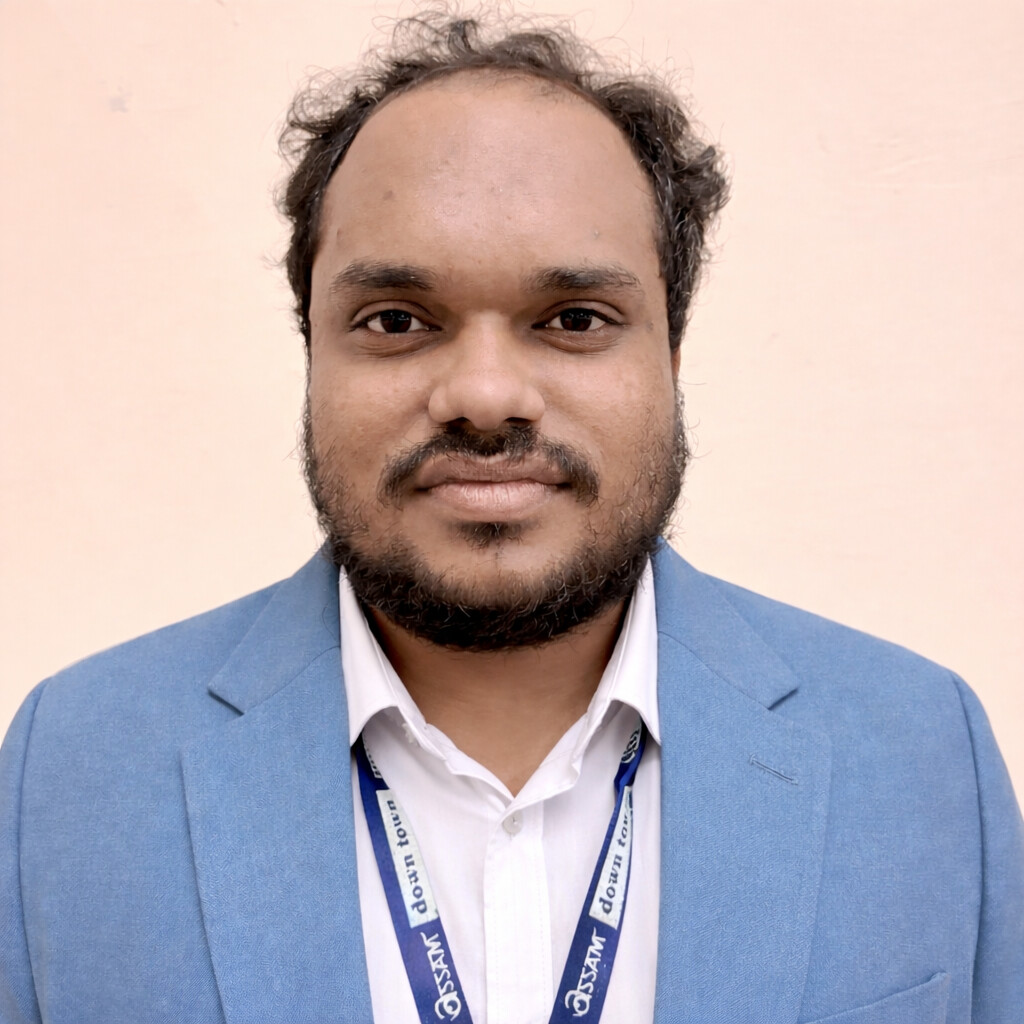
\includegraphics[width=\textwidth, height=0.15\textheight, keepaspectratio]{photo1.jpg}
    \end{minipage}%
    \begin{minipage}{0.7\textwidth}
        % \vspace*{0pt}
        \hspace*{4pt}
        \vspace*{4pt}
        {\Huge \scshape {Priya Raj Chanda}}\\
        \vspace*{2pt}
        {\color{emphcolor}\small\bfseries Assistant Professor
        \enspace|\enspace Computer Science \& Engineering}\\
        \vspace*{2pt}
        %\hspace*{10pt}
        %\faAngleDoubleRight AIML \& IoT Enthusiast \\
        \vspace*{2pt}
        \hspace*{2pt}
        \faEnvelope~\href{mailto:priyarajchanda@gmail.com}{priyarajchanda@gmail.com}\\
        \vspace*{2pt}
        \hspace*{2pt}
        \faPhone~\href{tel:+91 70029 69004}{+91 70029 69004}\\
        \vspace*{2pt}
        \hspace*{2pt}
        \faBirthdayCake \hspace{0.5pt} 05/06/1998\\
        \vspace*{2pt}
        \hspace*{2pt}
        \faMapMarker \hspace{0.5pt} Bhaskarnagar, Guwahati, Dist: Kamrup (M), Assam - 781018, India\\
        \vspace*{2pt}
        \hspace*{2pt}
        \textbf{\href{https://scholar.google.com/citations?user=nt04bqgAAAAJ&hl=en&authuser=2}{\textnormal{\aiGoogleScholar} \hspace{0.5pt} Google Scholar | }}
        \textbf{\href{https://orcid.org/0009-0006-4799-9757}{\textnormal{\aiOrcid} \hspace{0.5pt} ORCID | }}
        \textbf{\href{https://www.linkedin.com/in/priya-raj-chanda/}{\textnormal{\faLinkedin} \hspace{0.5pt} Linkedin | }}
        \textbf{\href{https://github.com/Priyoraj}{\textnormal{\faGithub} \hspace{0.5pt} Github}}
        %\textbf{\href{https://priyoraj.github.io/Portfolio/}{\faSuitcase \hspace{0.5pt} Portfolio}}\\
    \end{minipage}
\end{center}

\cvsection{Academic Profile}
Computer Science educator and researcher with undergraduate and postgraduate teaching experience and an M.Tech. in Computer Science \& Engineering (Artificial Intelligence). Research interests focus on machine learning, deep learning, computer vision, and the Internet of Things, with an emphasis on developing practical and intelligent solutions using AI-driven techniques. Dedicated to teaching, interdisciplinary research, and the application of emerging technologies to real-world problems.
\vspace{2mm}

      {\scshape\raggedright{\color{emphcolor}{Professional Appointments}}\par}\medskip
  \vspace{-\baselineskip}
  {\color{lightblue}\noindent\rule\linewidth{1.5pt} \par}
  \smallskip
      \vspace{0.5mm}
      Assistant Professor in the Programme of Computer Science \& Engineering (Faculty of Computer Technology) at \textbf{\href{https://adtu.in/teaching-faculties/TVRVNE1nPT0=/.html}{Assam down town University, Guwahati, Assam - 781026, India}} \hfill \faCalendar \hspace{0.5pt} 15 September 2025 - Present\\
      \begin{itemize}
          \item In my capacity at this university, I serve as a member of the departmental lab committee as well as the Faculty Course Coordinator for the following undergraduate \& postgraduate courses:
          \vspace*{1mm} \\
            \begin{tabular}[t]{@{}>{\raggedright\arraybackslash}p{0.48\linewidth}@{\hspace{0.04\linewidth}}>{\raggedright\arraybackslash}p{0.48\linewidth}@{}}
            1. Fundamentals of AI / ML (24MCAM2105R) & 2. Problem Solving Using C (BTCS1101) \\
            3. Social Network Analysis (22BTCS414R) & 4. Artificial Intelligence (24BCSM2204R) \\
            5. Internet of Things (23BTCS3205R) & 6. Data Structure \& Algorithms (BCST1203) \\
            7. Data Communication \& Computer Network (24BCSM3101R) & 8. Programming With Python (BTCS2101)
        \end{tabular}
      \end{itemize}
      
      \vspace{0.5mm}
       \vspace{0.5mm}

      Assistant Professor in the Department of Computer Science \& Engineering at \textbf{\href{https://drive.google.com/file/d/1epEgTLdh-mOB0pqq_2WUmILy305SlNiP/view?usp=sharing}{Academy of Technology, Hooghly, West Bengal - 712121, India}} \hfill \faCalendar \hspace{0.5pt} 28 February 2023 - 14 June 2024\\
      \begin{itemize}
          \item In my capacity at this institution, I served as the departmental MAR \& MOOCS Coordinator as well as the Faculty Course Coordinator for the following undergraduate courses:
          \vspace*{1mm} \\
            \begin{tabular}[t]{@{}>{\raggedright\arraybackslash}p{0.48\linewidth}@{\hspace{0.04\linewidth}}>{\raggedright\arraybackslash}p{0.48\linewidth}@{}}
            1. Introduction to Internet of Things & 2. Programming for Problem Solving \\
            3. E-Commerce \& ERP & 4. Computer Networks Lab \\
            5. Fundamentals of Computer Science Lab &
        \end{tabular}
      \end{itemize}
      
      \vspace{0.5mm}
%%%%%%%%%%%%%%%%%%%%%%%%%%%%%%%%%%%%%%
    %
    %     Education
    %
    %%%%%%%%%%%%%%%%%%%%%%%%%%%%%%%%%%%%%%
      %\header{Education}
      %\medskip
  {\scshape\raggedright{\color{emphcolor}{Education}}\par}\medskip
  \vspace{-\baselineskip}
  {\color{lightblue}\noindent\rule\linewidth{1.5pt} \par}
  \smallskip
  \vspace{0.5mm}
%    \textbf{\faUniversity \hspace{0.5pt} Indian Institute of Information Technology Guwahati}\hfill \faMapMarker \hspace{0.5pt} Assam, India\\
% Ph. D. in Computer Science \& Engineering \hfill August 2024 - Present
% \\
\vspace*{4pt}
      \textbf{\textnormal{\faUniversity} \hspace{0.5pt} Centre For Development of Advanced Computing, Mohali}\hfill \faMapMarker \hspace{0.5pt} Punjab, India\\
M. Tech. in Computer Science \& Engineering (Artificial Intelligence) \hfill August 2021 - June 2024
\\
{\sl CGPA: 8.03 out of 10}\\
\vspace*{4pt}
      \textbf{\textnormal{\faGraduationCap} \hspace{0.5pt} Central Institute of Technology, Kokrajhar}\hfill \faMapMarker \hspace{0.5pt} Assam, India\\
B. Tech. in Information Technology \hfill July 2016 - August 2021
\\
{\sl CGPA: 7.54 out of 10}\\
\vspace*{4pt}
      \textbf{\textnormal{\faBook} \hspace{0.5pt} Shrimanta Shankar Academy, Panbazar}\hfill \faMapMarker \hspace{0.5pt} Assam, India\\
10+2 Science \hfill July 2014 - June 2016
\\
{\sl Percentage: 68.8}\%\\
\vspace*{4pt}
      \textbf{\textnormal{\faBook} \hspace{0.5pt} Don Bosco School, Sonaighuli}\hfill \faMapMarker \hspace{0.5pt} Assam, India\\
HSLC \hfill January 2002 - June 2014
\\
{\sl Percentage: 77.3}\%\\
\vspace*{2mm}

{\scshape\raggedright{\color{emphcolor}{Publication}}\par}\medskip
  \vspace{-\baselineskip}
  {\color{lightblue}\noindent\rule\linewidth{1.5pt} \par}
  \smallskip
      \vspace{0.5mm}
      Amitava Nag, \textbf{Priya Raj Chanda}, and Sukumar Nandi. "Mobile app-based tomato disease identification with fine-tuned convolutional neural networks." Computers and Electrical Engineering 112 (2023): 108995.
      \newline\textbf{DOI: }{\em \href{https://doi.org/10.1016/j.compeleceng.2023.108995}{https://doi.org/10.1016/j.compeleceng.2023.108995}}
      \vspace*{14mm}\\

 {\scshape\raggedright{\color{emphcolor}{Research Interests \& Technical Skills}}\par}\medskip
  \vspace{-\baselineskip}
  {\color{lightblue}\noindent\rule\linewidth{1.5pt} \par}
  \smallskip
  \vspace{0.5mm}
  \begin{longtable}{p{4cm}p{12cm}}
  Research Interests: & Computer Vision, Machine Learning, Deep Learning, Internet of Things \\
  Programming: & C, C++, Python, JavaScript, WebAssembly \\
  Libraries \& tools: & PyTorch, Fast.ai, IceVision, Tensorflow, Keras \\
  Typesetting: & \LaTeX
  \end{longtable}
  \vspace{0.5mm}


      {\scshape\raggedright{\color{emphcolor}{Projects}}\par}\medskip
  \vspace{-\baselineskip}
  {\color{lightblue}\noindent\rule\linewidth{1.5pt} \par}
  \smallskip
      \vspace{0.5mm}
      {\textbf{PaperBot: Automated Research-Paper Request Assistant}}\hfill{\href{https://github.com/Priyoraj/paperbot}{\faGithub \hspace{0.5pt} github.com/Priyoraj/paperbot}}\\
      {\sl Python, Tkinter, Playwright, SQLite, IMAP/SMTP}\\
          \vspace{-3mm}
\begin{itemize} \itemsep -3pt
\item Desktop app that answers colleagues' paper requests by e-mail: finds each paper (Crossref, arXiv, Semantic Scholar), sends open-access copies first, and uses institutional VPN access only within daily fair-use limits.
\item Handles approval of new requesters, a queue for papers that need a manual download, and several computers sharing one mailbox; covered by 150+ automated tests.
\end{itemize}
          \vspace*{0.5mm}
      {\textbf{FoCT Virtual Labs: Browser-based Computer Labs}}\hfill{\href{https://github.com/Priyoraj/foct-virtual-labs}{\faGithub \hspace{0.5pt} github.com/Priyoraj/foct-virtual-labs}}\\
      {\sl Python, JavaScript, WebAssembly}\hfill{\href{https://priyoraj.github.io/foct-virtual-labs/}{\faGlobe \hspace{0.5pt} Live demo: priyoraj.github.io/foct-virtual-labs}}\\
          \vspace{-3mm}
\begin{itemize} \itemsep -3pt
\item Built for the Faculty of Computer Technology, Assam down town University: labs for C, C++, Python/Jupyter, Java, SQL, MongoDB, compiler design, circuit and network simulation, and packet analysis.
\item Compilers and runtimes run as WebAssembly in each student's browser, so one ordinary PC serves a whole lab offline.
\item Exam mode with copy/paste lock, watermarking, collection of students' work and a code-similarity report; load-tested with 500 simultaneous clients.
\end{itemize}
          \vspace*{0.5mm}
      {\textbf{crypto-web: Encryption \& Decryption Web Application}}\hfill{\href{https://github.com/Priyoraj/crypto-web}{\faGithub \hspace{0.5pt} github.com/Priyoraj/crypto-web}}\\
      {\sl JavaScript, HTML, CSS}\hfill{\href{https://priyoraj.github.io/crypto-web/}{\faGlobe \hspace{0.5pt} Live demo: priyoraj.github.io/crypto-web}}\\
          \vspace{-3mm}
\begin{itemize} \itemsep -3pt
\item Teaching tool for the Caesar, Playfair and DES / Triple-DES ciphers that shows the Playfair key square and every round of DES; runs in any browser without installation.
\end{itemize}
          \vspace*{0.5mm}
{\scshape\raggedright{\color{emphcolor}{Professional Development \& Certifications}}\par}\medskip
  \vspace{-\baselineskip}
  {\color{lightblue}\noindent\rule\linewidth{1.5pt} \par}
  \smallskip
      \vspace{0.5mm}
{\small Faculty development programmes (FDPs), workshops, and training.\par}
      \vspace{2mm}
      • \href{https://drive.google.com/file/d/1EiFM5zp710JMe26lP_MTdjMw3ejmifCT/view?usp=drive_link}{FDP on Generative AI \& Agentic AI: Transforming Teaching, Research, and Innovation in Higher Education - \textbf{Assam down town University}}\\
\vspace*{1mm}
      • \href{https://drive.google.com/file/d/1OChnYzTUL_kv7vNiY-iNZFfVF7Yy-fP-/view}{FDP on Quantum Computing Foundations and Applications - \textbf{Assam down town University}}\\
\vspace*{1mm}
%       • \href{https://drive.google.com/file/d/1ZnYxLv5BMT7kqaCPsxcxafg86vTerdig/view} {Resource Person for Skill Development Program on Basic Computer Applications - \textbf{Assam down town University \& Rotary Club of Guwahati}}\\
% \vspace*{1mm}
      • \href{https://drive.google.com/file/d/1GkauKiD-faksW_H-e1YVG0FRoTd1Y6Gw/view}{Industry Academia Engagement Workshop on Hardware Accelerators for Neural Network Applications - \textbf{IIT Guwahati \& IEEE Kolkata Section }}\\
\vspace*{1mm}
      • \href{https://drive.google.com/file/d/1hxyq4EwJViLteH_s38yKJDIG6zEyN-yw/view?usp=sharing}{FDP on Recent Advancement \& Future Trends in AI and ML (RAFTML) - \textbf{Abacus Institute of Engineering And Management, Hooghly, West Bengal }}\\
\vspace*{1mm}
      • \href{https://drive.google.com/file/d/1nkywl5fc3onvEmR8JhIFHx_8UYcwEUbY/view?usp=sharing}{FDP on Internet of Things (IoT) with Artificial Intelligence (AI) and Machine Learning (ML) - \textbf{Academy of Technology, Hooghly, West Bengal }}\\
\vspace*{1mm}
      • \href{https://drive.google.com/file/d/14PB8_c5nCV9akWrfmdYdHLCoCkthIhet/view?usp=sharing}{Fellow at 6th Summer School on Artificial Intelligence with focus on Computer Vision \& Machine Learning - \textbf{IIIT Hyderabad}}\\
\vspace*{1mm}
      • \href{https://drive.google.com/file/d/1qrwGlTguMqHuLFoG9R3_M4pFOLr7850p/view?usp=sharing}{Project-based online course on Machine Learning Using Python - \textbf{Skyfilabs}}\\
\vspace*{1mm}
      • \href{https://drive.google.com/file/d/1PJgvEGv3F3bIdsVFiNCZsQhPgqEcOGZf/view?usp=sharing}{Project-based Industrial Training Program on Web Development using Python - \textbf{OgmaTechLab}}\\
\vspace*{1mm}
      • \href{https://drive.google.com/file/d/1H-Ha-RE7amy0kRLSrc0BiSP4dSCIaA6K/view?usp=sharing}{Internet of Things (IoT) \& Its Applications - \textbf{CIT Kokrajhar ACM Student Chapter}}\\
\vspace*{1mm}
      • \href{https://drive.google.com/file/d/1ZxBTVE3T-Dbd9iVSJZ-SoHss1sIOy5Yj/view?usp=sharing}{Python Scripting and Security - \textbf{Techcracy 2016}}\\
\vspace*{2mm}

{\scshape\raggedright{\color{emphcolor}{Leadership \& Academic Service}}\par}\medskip
  \vspace{-\baselineskip}
  {\color{lightblue}\noindent\rule\linewidth{1.5pt} \par}
  \smallskip
      \vspace{0.5mm}
      • \href{https://drive.google.com/file/d/1ZnYxLv5BMT7kqaCPsxcxafg86vTerdig/view} {\textbf{Resource Person}, Skill Development Program on Basic Computer Applications - \textbf{Assam down town University \& Rotary Club of Guwahati}}\\
\vspace*{1mm}
      • \textbf{Student Member \& Treasurer}, Association for Computing Machinery (ACM) Student Chapter - \textbf{Central Institute of Technology, Kokrajhar}
    \vspace{5mm} 
      \\ \textbf{\em{I declare that the information furnished above is true to the best of my knowledge.
       \\ \hfill-Priya Raj Chanda}}
      
\end{document}